\section{Appendix: Foundations}
\subsection{Important functions}
\subsubsection{Rectified Linear Unit}
Properties of the ReLU function:
\begin{itemize}
	\item $\text{ReLU}(x)=\max(x,0)$
	\item $\text{ReLU}'(x)=\begin{cases}
	1 & \text{ if } x>0\\
	0 & \text{ if } x<0\\
	\text{undef} & \text{ if } x=0\\
	\end{cases}$ (last case usually set to 0)
	\item Variations: 
	\begin{itemize}
		\item Leaky ReLU: $f(x)=\begin{cases}
		x & \text{ if } x>0\\
		0.01x & \text{ otherwise }
		\end{cases}$
		\item ELU: $f(x)=\begin{cases}
		x & \text{ if } x>0\\
		\alpha (e^x-1) & \text{ otherwise }
		\end{cases}$
		\item Self-normalizing ELU (carefully selected $\alpha$ and scaling, so that activations stay close to mean 0, variance 1)
	\end{itemize}
\end{itemize}
\subsubsection{Sigmoid}
Properties of the sigmoid function:
\begin{itemize}
	\item $\sigma(x)=\frac{1}{1+e^{-x}}$
	\item $\sigma(-x) = 1 - \sigma(x)$
	\item $\sigma'(x) = \sigma(x)\left(1 - \sigma(x)\right)$
	\item Output range: $[0,1]$
\end{itemize}
\begin{figure}[ht]
	\centering
	\begin{subfigure}[b]{0.3\textwidth}
		\centering
		\scalebox{0.5}{%
			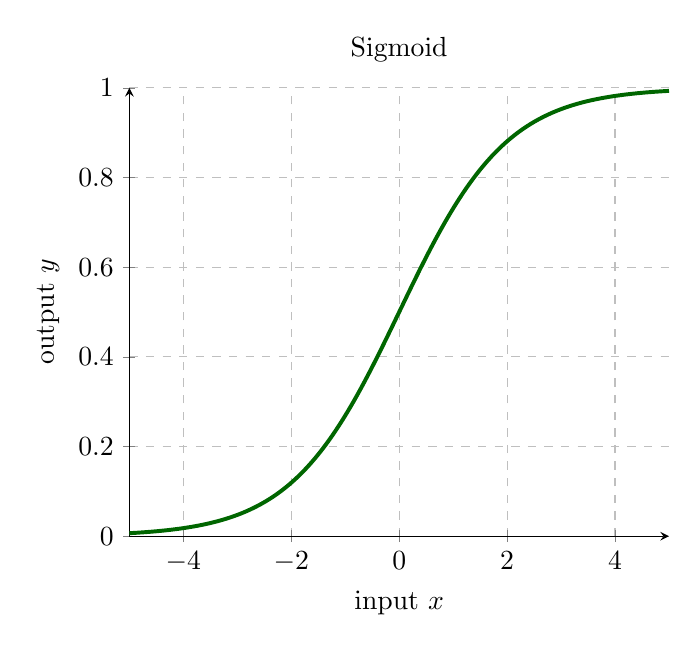
\begin{tikzpicture}
			\begin{axis}[
			title = {Sigmoid},
			axis lines = left,
			xlabel = {input $x$},
			ylabel = {output $y$},
			xmin = -5,
			xmax = 5,
			ymin = 0,
			ymax = 1,
			ymajorgrids=true,
			xmajorgrids=true,
			grid style=dashed
			]
			%Here the blue parabloa is defined
			\addplot [
			domain=-5:5, 
			samples=1000, 
			color=black!60!green,
			line width = 0.5mm
			]
			{1/(1+e^(-x))};
			
			\end{axis}
			\end{tikzpicture}
		}
		\caption{$\sigma(x)$}
		\label{img:activation_function_sigmoid}
	\end{subfigure}
	\begin{subfigure}[b]{0.3\textwidth}
		\centering
		\scalebox{0.5}{%
			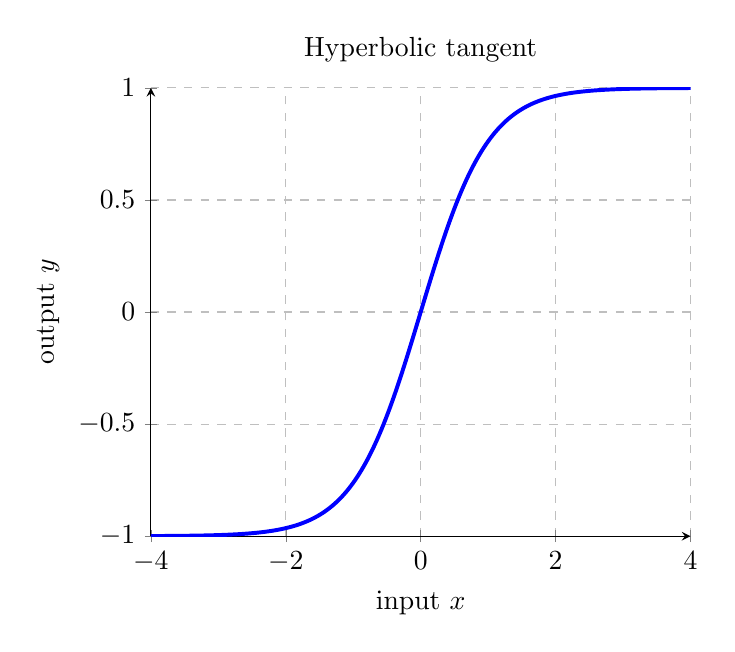
\begin{tikzpicture}
			\begin{axis}[
			title = {Hyperbolic tangent},
			axis lines = left,
			xlabel = {input $x$},
			ylabel = {output $y$},
			xmin = -4,
			xmax = 4,
			ymin = -1,
			ymax = 1,
			ymajorgrids=true,
			xmajorgrids=true,
			grid style=dashed
			]
			%Here the blue parabloa is defined
			\addplot [
			domain=-4:4, 
			samples=1000, 
			color=blue,
			line width = 0.5mm
			]
			{tanh(x)};
			
			\end{axis}
			\end{tikzpicture}
		}
		\caption{$\tanh(x)$}
		\label{img:activation_function_tanh}
	\end{subfigure}
	\begin{subfigure}[b]{0.3\textwidth}
		\centering
		\scalebox{0.5}{%
			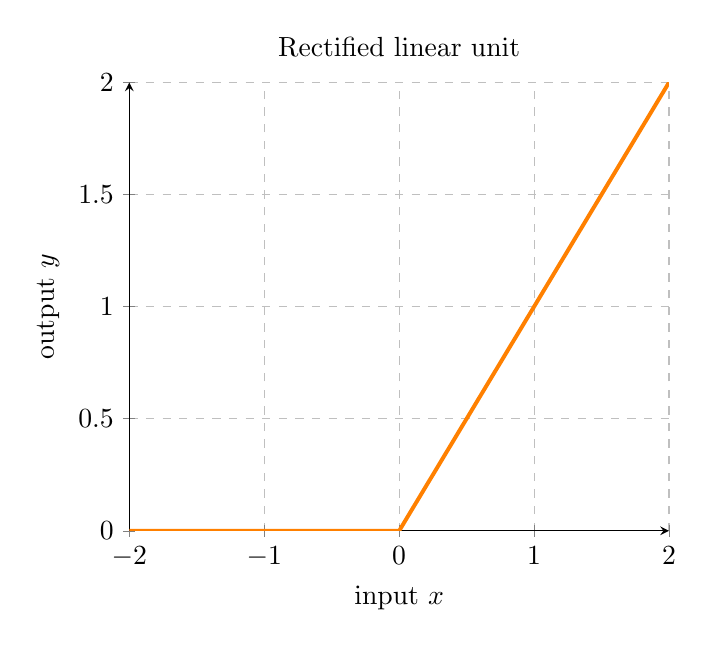
\begin{tikzpicture}
			\begin{axis}[
			title = {Rectified linear unit},
			axis lines = left,
			xlabel = {input $x$},
			ylabel = {output $y$},
			xmin = -2,
			xmax = 2,
			ymin = 0,
			ymax = 2,
			ymajorgrids=true,
			xmajorgrids=true,
			grid style=dashed
			]
			%Here the blue parabloa is defined
			\addplot [
			domain=-2:2, 
			samples=1000, 
			color=orange,
			line width=0.5mm
			]
			{(x > 0)*x};
			
			\end{axis}
			\end{tikzpicture}
		}
		\caption{$\text{ReLU}(x)$}
		\label{img:activation_function_relu}
	\end{subfigure}
	
	\caption[Comparison of activation functions]{(a) The sigmoid function maps the inputs to a range of 0 to 1 while having high gradients near to $y=0$ to bring the output more to either 0 or 1. (b) The hyperbolic tangent is similar to the sigmoid function but has a output range of -1 to 1. (c) A rectified linear unit (ReLU) is 0 for all input lower than 0. All other values are processed linearly so that they do not change.}
\end{figure}
\subsubsection{Hyperbolic tan}
Properties of the hyperbolic tan:
\begin{itemize}
	\item $\tanh(x) = \frac{e^{x} - e^{-x}}{e^{x} + e^{-x}}$
	\item $\tanh(-x) = -\tanh(x)$
	\item $\tanh'(x) = 1 - \tanh(x)^2$
	\item Output range: $[-1,1]$
\end{itemize}
\subsubsection{Softmax}
Properties:
\begin{itemize}
	\item $\text{softmax}(x_k) = \frac{\exp(x_k)}{\sum_{i=1}^{N}\exp(x_i)}$
	\item If $x_k \gg x_j$, the softmax for all $j\neq k$ is approx. 0, whereas for $k$ it is 1
	\item Maps vector from $\bm{y} \in \mathbb{R}^D$ to probability distribution $\bm{y}' \in [0,1]^D$ with $\sum_{i=1}^{D}y'_{i} = 1$ $\Rightarrow$ useful for multi-class classification
	\item Invariant to bias: $\frac{\exp(x_k + c)}{\sum_{i=1}^{N}\exp(x_i + c)} = \frac{\exp(x_k)}{\sum_{i=1}^{N}\exp(x_i)}= \text{softmax}(x_k)$
\end{itemize}
\subsection{Matrix operations}
\subsubsection{Properties of transposed and inverse matrices}
\textbf{Transpose}
\begin{itemize}
	\item $(AB)^T=B^T A^T$
	\item $\det\left(A^{T}\right) = \det\left(A\right)$
\end{itemize}
\textbf{Inverse}
\begin{itemize}
	\item $(AB)^{-1} = B^{-1} A^{-1}$
	\item $\det\left(A^{-1}\right) = \det\left(A\right)^{-1}$
\end{itemize}
\textbf{Combination}
\begin{itemize}
	\item $\left(A^{-1}\right)^T = \left(A^{T}\right)^{-1}$
\end{itemize}
\subsubsection{Derivations}
\subsubsection{Hand-in 1: 1.3d}
Derivation of multivariate Gaussian by matrix
\subsection{Lagrange Multiplier}
\begin{itemize}
	\item Finding stationary points of a function with subject to one or more constraints
	\item \textbf{Equality constraint}
	\begin{itemize}
		\item Maximize $f(\bm{x})$ with respect to constraint $g(\bm{x})=0$
		\item At a constrained maximum, we know that $\nabla f(\bm{x}) = -\lambda \nabla g(\bm{x})$
		\item The Lagrangian function is therefore $$ L(\bm{x}, \lambda) = f(\bm{x}) + \lambda g(\bm{x})$$
		\item We solve it by maximizing regarding to $\bm{x}$ and $\lambda$: $$\max_{\bm{x}} \max_{\lambda} L(\bm{x}, \lambda)$$
		\item Note that the sign of the constraint is irrelevant. A minus sign leads to the same result as $g(x)$ must be zero at this point
		\item We find solutions by setting the derivate of both primal and dual variables to 0:
		$$\frac{\partial }{\partial \bm{x}} L(\bm{x}, \lambda) = 0, \text{\hspace{3mm}} \frac{\partial }{\partial \lambda} L(\bm{x}, \lambda) = 0$$
	\end{itemize}
	\item \textbf{Inequality constraint}
	\begin{itemize}
		\item Maximize $f(\bm{x})$ with respect to constraint $g(\bm{x})\geq0$ (introduce Lagrangian multiplier $\mu$)
		\item Two kinds of solutions:
		\begin{itemize}
			\item If the optimum of $f(\bm{x})$ lies already in the region of $g(\bm{x})\geq0$, then we have an inactive constraint $\Rightarrow$ $\mu=0$
			\item Otherwise, the optimum is on the boundary so that $g(\bm{x})=$ and $\mu> 0$
		\end{itemize}
		\item Thus, our primal Lagrangian is defined as:
		$$L(\bm{x}, \mu) = f(\bm{x}) + \mu g(\bm{x})$$
		\item We now maximize regarding $\bm{x}$, but \textit{minimize} for the Lagrangian multiplier as we prefer $f(x)$ being inside the constraint area:
		$$\max_{\bm{x}} \min_{\mu} L(\bm{x}, \mu)$$
		\item Note that the sign is here important. When we minimize $f(x)$, we can keep the max-min conditions for the Lagrangian but then have to switch the sign in front of the constraint!
		\item Also, deriving by $\mu$ does not guarantee a valid solution anymore as we have the following KKT conditions for \textit{every} Lagrangian multiplier:
		$$\mu \geq 0 \hspace{5mm} g(\bm{x})\geq 0 \hspace{5mm} \mu g(\bm{x}) = 0$$
		\item We obtain the dual Lagrangian by optimizing with respect to only the primal variables $\bm{x}$, and replacing those in the primal Lagrangian:
		$$\tilde{L}(\mu) = \max_{\bm{x}} L(\bm{x},\mu)$$
		\item Next, minimize with respect to the dual parameters $\mu$ by considering the constraint $\mu=0$
	\end{itemize}
	\item \textbf{Combined constraints}
	\begin{itemize}
		\item If we have multiple constraints (can be pure (in-)equalities or mixed), we just add them all to our Lagrangian function
		\item Solve with respect to all constraints
	\end{itemize}
\end{itemize}